\section{Inter-GPU communication without CPU Intervention}
In this section, we talk about GPUDirect technology for communicating between GPUs without any CPU intervention via Remote Dynamic Memory Access (RDMA). Then we talk about our attempt of implementing the GPUDirect technology in the Gluon communication substrate. We further discuss about the challenges that we faced in this implementation and our insights. 

\subsection{GPUDirect Technology}
Message Passing Interface (MPI) is a standard API for communicating data via messages between distributed processes that is commonly used in High Performance Computing (HPC) to build applications that can scale to multi-node compute clusters. The MPI standard defines a message-passing API which covers point-to-point messages as well as collective operations like reductions. 

\begin{figure}
\centering
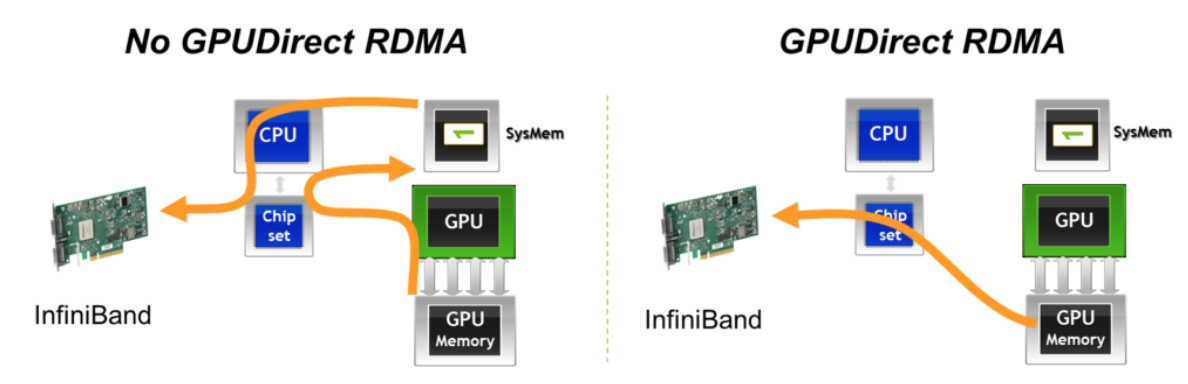
\includegraphics[width=0.49\textwidth]{gpu-rdma.png}
\mycaption{GPUDirect RDMA}{The figure shows the data transfers with and without GPUDirect RDMA. 
}
\label{fig-rdma}
%\vspace{-20pt}
\end{figure}

\begin{figure}
\centering
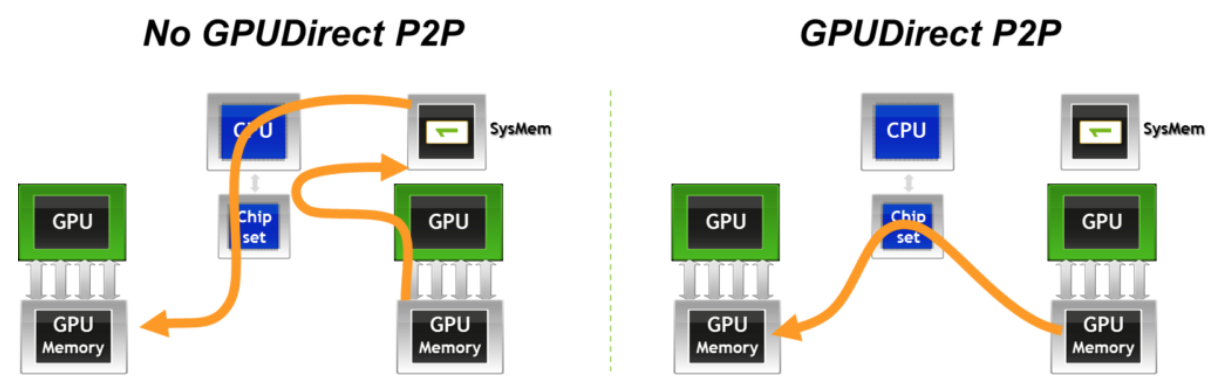
\includegraphics[width=0.49\textwidth]{gpu-ptp.png}
\mycaption{GPUDirect Peer-to-Peer}{The figure shows the data transfers with and without GPUDirect Peer-to-Peer. 
}
\label{fig-ptp}
%\vspace{-20pt}
\end{figure}


NVIDIA GPUDirect technologies provide high-bandwidth, low-latency communications with NVIDIA GPUs. GPUDirect is an umbrella name used to refer to several specific technologies. In the context of MPI the GPUDirect technologies cover all kinds of inter-rank communication: intra-node, inter-node, and RDMA inter-node communication. The newest GPUDirect feature is support for Remote Direct Memory Access (RDMA), with which buffers can be directly sent from the GPU memory to a network adapter without staging through host memory. This is shown in Figure~\ref{fig-rdma}. Another variant is GPUDirect for Peer-to-Peer (P2P) transfers, which can accelerate intra-node communication. Buffers can be directly copied between the memories of two GPUs in the same system with GPUDirect P2P. This is shown in Figure~\ref{fig-ptp}. 

If GPUDirect RDMA or GPUDirect P2P is available, the buffers can be directly transferred from the source to the destination without touching the host memory at all. This saves a lot of overhead in serializing/deserializing data and also copying of data between CPU and GPU buffers. Furthermore, the GPUDirect technology can be used along with Unified Virtual Addresses, which further eases the implementation as we do not have to worry about the location of the buffers that are being transferred. 

\subsection{GPUDirect in Gluon}
We attempted to implement the GPUDirect P2P and GPUDirect RDMA transfers on the Gluon Substrate, for transferring the data between GPUs of a single node in the context of the bfs\_push application. As explained before, when a source node tries to transfer data to a destination node, the following steps occur:
\begin{enumerate}
\item The offset data and the bitset data of the updated nodes are computed at the GPU of the source
\item The offset data, bitset data and the updated node label data are copied and serialized into a CPU buffer at the source
\item The CPU buffer is transferred using MPI from the source
\item The CPU buffer is received using MPI at the destination
\item The CPU buffer at the destination is deserialized and copied to the GPU at the destination
\end{enumerate}
Using the GPUDirect Technology in this workflow, we can greatly reduce the overheads in these transfers, to the following steps:
\begin{enumerate}
\item The offset data and the bitset data of the updated nodes are computed at the GPU of the source
\item The offset data, bitset data and the updated node label data are serialized and transferred directly from the source GPU using MPI
\item The offset data, bitset data and the updated node label data are directly received at the destination GPU using MPI
\item The received data is deserialized and scattered to the proper location of GPU memory
\end{enumerate}
Note that all the steps can occur simultaneously along with other computations at the CPU of source and destination. The GPU-GPU data transfers occur asynchronously without any CPU involvement. This feature, if applied effectively, has the potential to significantly improve the performance of data transfers, as compared to the other two features.

\subsection{Discussion and Limitations}
The current Gluon substrate networking works like below.
\begin{enumerate}
\item Background thread catches and polls all OpenMPI messages received on the node.
\item During the MPI communication, all the MPI messages are sent or received asynchronously.
CPU buffers which are completely received through these messages are scattered across the vector of the buffer vector.
Indices for this vector represents host IDs. For example, 1th buffer vector stores received buffers from the host 1.
\item For each round of BFS, the Gluon substrate iterates the buffer vectors checks whether there is any completely received buffer or not.
If there is, the buffer is popped from the deserialized, and, copied to and scattered across GPU memory. 
\end{enumerate}
The main challenge that we have faced while applying GPUDirect technology is that Gluon substrate collects messages on CPU, not GPU. 
To make it receive MPI message on GPU, we should modify entire Gluon substrate implementation.
First, we should the CPU worker thread ignore the GPUDirect message. 
Todo this, we fix the GPUDirect message tag to 10000. 
When any message whose tag is 10000 arrives, the worker thread probes and ignore it.
Second, we put GPUDirect send and receive parts on GPU side. 
The message ignored by the worker tread finally are received by GPUDirect receive code.
Since we cannot exploit the worker thread, we use synchronous (blocking) MPI receive.
Finally, we replaced the previous deserialization/serialization/copy/scatter of CPU-GPU codes with 
deserialization/serialization/scatter of GPU-GPU codes. In this case, we also apply asynchronous memory copy 
and UVA technologies.

Due to the current limitation of Gluon substrate, 
we could not fully apply GPUDirect technologies.
However, in the future, we expect that we can support full GPUDirect by replacing the network interface. 










